\documentclass[12pt,a4paper]{article}

%% ── Packages ─────────────────────────────────────────────────────────────────
\usepackage[T1]{fontenc}
\usepackage[utf8]{inputenc}
\usepackage{lmodern}
\usepackage[margin=2.5cm]{geometry}
\usepackage{graphicx}
\usepackage{xcolor}
\usepackage{hyperref}
\usepackage{booktabs}
\usepackage{longtable}
\usepackage{array}
\usepackage{enumitem}
\usepackage{caption}
\usepackage{float}
\usepackage{amsmath}
\usepackage{tikz}
\usetikzlibrary{shapes.geometric,arrows.meta,positioning,fit,backgrounds,calc}
\usepackage{fancyhdr}
\usepackage{titlesec}
\usepackage{parskip}
\usepackage{microtype}
\usepackage{tcolorbox}
\tcbuselibrary{skins,breakable}

%% ── Colours ──────────────────────────────────────────────────────────────────
\definecolor{cmuRed}{RGB}{196,18,48}
\definecolor{codeGray}{RGB}{245,245,245}
\definecolor{linkBlue}{RGB}{0,70,180}
\definecolor{attackRed}{RGB}{200,30,30}
\definecolor{defenseGreen}{RGB}{20,130,60}

%% ── Hyperref ─────────────────────────────────────────────────────────────────
\hypersetup{
  colorlinks=true, linkcolor=linkBlue,
  urlcolor=linkBlue, citecolor=linkBlue,
  pdftitle={MedVault -- Secure Medical Records System},
  pdfauthor={CMU Information Security -- Spring 2026},
}

%% ── Section style ────────────────────────────────────────────────────────────
\titleformat{\section}{\large\bfseries\color{cmuRed}}{\thesection}{1em}{}[\titlerule]
\titleformat{\subsection}{\normalsize\bfseries\color{cmuRed!80!black}}{\thesubsection}{1em}{}

%% ── Header / footer ──────────────────────────────────────────────────────────
\pagestyle{fancy}\fancyhf{}
\lhead{\small\textcolor{cmuRed}{\textbf{MedVault}} -- Secure Medical Records}
\rhead{\small CMU InfoSec -- Spring 2026}
\cfoot{\thepage}
\renewcommand{\headrulewidth}{0.4pt}

%% ── Coloured boxes ───────────────────────────────────────────────────────────
\newtcolorbox{attackbox}{colback=red!5!white,colframe=attackRed,
  fonttitle=\bfseries,title=Attack Scenario,breakable,enhanced}
\newtcolorbox{defensebox}{colback=green!5!white,colframe=defenseGreen,
  fonttitle=\bfseries,title=Defense Implemented,breakable,enhanced}
\newtcolorbox{notebox}{colback=blue!5!white,colframe=linkBlue,
  fonttitle=\bfseries,title=Note,breakable,enhanced}

%% ── File-reference helper ────────────────────────────────────────────────────
%% \srcref{display}{path}  -- typesets path as a clickable footnote
\newcommand{\srcref}[2]{\texttt{#1}\footnote{Full source: \texttt{#2}}}

%% ── TikZ helpers ─────────────────────────────────────────────────────────────
\tikzset{
  layer/.style={draw,rounded corners=3pt,minimum width=9cm,minimum height=0.85cm,
                font=\small\bfseries,align=center,text width=8.6cm},
  mod/.style={draw,rounded corners=3pt,minimum width=2.2cm,minimum height=0.75cm,
              font=\scriptsize\bfseries,align=center,fill=blue!8},
  sbox/.style={draw,rounded corners=3pt,minimum width=2.6cm,minimum height=0.75cm,
               font=\scriptsize,align=center,fill=gray!8},
  diam/.style={draw,diamond,aspect=2.2,font=\scriptsize,align=center,fill=yellow!15},
  state/.style={draw,rounded corners=4pt,minimum width=2.2cm,minimum height=0.75cm,
                font=\scriptsize\bfseries,align=center},
  threat/.style={draw,rounded corners=3pt,minimum width=2.8cm,minimum height=0.9cm,
                 font=\scriptsize\bfseries,align=center},
  arr/.style={-Stealth,thick},
  darr/.style={-Stealth,thick,gray!60},
}

%% =============================================================================
\begin{document}

%% ── Title page ───────────────────────────────────────────────────────────────
\begin{titlepage}
  \centering\vspace*{2cm}
  {\Huge\bfseries\color{cmuRed}MedVault}\\[0.4cm]
  {\Large Secure Medical Records System}\\[0.2cm]
  {\large\textit{Final Project Report}}\\[2cm]
  
\begin{tikzpicture}
    \fill[cmuRed!15](0,0)--(2.5,0)--(2.5,2.8)--(1.25,3.8)--(0,2.8)--cycle;
    \draw[cmuRed,line width=2pt](0,0)--(2.5,0)--(2.5,2.8)--(1.25,3.8)--(0,2.8)--cycle;
    \node[font=\Large\bfseries,text=cmuRed] at (1.25,1.8){MV};
    \draw[cmuRed!60,line width=1pt](0.5,0.8)--(2.0,0.8);
    \draw[cmuRed!60,line width=1pt](0.5,1.2)--(2.0,1.2);
  \end{tikzpicture}\\[2cm]
  {\large Carnegie Mellon University}\\[0.2cm]
  {\large Information Security -- Spring 2026}\\[2cm]
  \begin{tabular}{rl}
    \textbf{Course:}   & Information Security \\
    \textbf{Project:}  & Secure Medical Records Backend \\
    \textbf{Language:} & Python 3.11+ / FastAPI / PostgreSQL \\
    \textbf{Date:}     & April 2026 \\
  \end{tabular}
  \vfill
  \textit{System architecture \textbullet{} Threat model \textbullet{}
          Secure protocol design \textbullet{} Prototype \textbullet{}
          Attack \& defence demos}
\end{titlepage}

\tableofcontents\newpage

%% =============================================================================
\section{Introduction}
%% =============================================================================

\textbf{MedVault} is a production-grade secure medical records backend designed
for Rwandan healthcare institutions. It provides authenticated, role-gated,
consent-controlled access to encrypted patient records, backed by a
tamper-evident audit trail on every sensitive operation.

The system was built as a final project for the CMU Information Security course
(Spring 2026) and demonstrates the full security engineering lifecycle:
requirements analysis, threat modelling, secure protocol design, implementation,
and adversarial testing.

\subsection{Objectives}
\begin{itemize}[leftmargin=1.5em]
  \item Design a secure system architecture with clear trust boundaries.
  \item Apply cryptographic primitives correctly (AES-256-GCM, bcrypt, HMAC-SHA1 TOTP).
  \item Build secure APIs with JWT + TOTP multi-factor authentication.
  \item Conduct structured threat modelling using STRIDE.
  \item Demonstrate 11 attack scenarios and their corresponding defences.
\end{itemize}

\subsection{Technology Stack}
\begin{center}
\begin{tabular}{ll}
  \toprule
  \textbf{Component} & \textbf{Technology} \\
  \midrule
  Web framework   & FastAPI (Python 3.11+) \\
  Database        & PostgreSQL 15+ (asyncpg) \\
  ORM             & SQLAlchemy 2.x (async) \\
  Authentication  & JWT HS256 + custom RFC~6238 TOTP \\
  Encryption      & AES-256-GCM (\texttt{cryptography} library) \\
  Password hashing& bcrypt \\
  Transport       & TLS 1.2+ (self-signed for dev) \\
  Migrations      & Alembic \\
  Testing         & pytest + Hypothesis \\
  \bottomrule
\end{tabular}
\end{center}

%% =============================================================================
\section{System Architecture}
%% =============================================================================

\subsection{Layered Architecture with Trust Boundaries}

MedVault uses a strict layered architecture. Each layer enforces its own
security controls independently, so a bypass at one layer does not grant access
to the next.

%% INSERT PHOTO HERE
%% Type: screenshot of the running system / browser showing register page
%% Caption suggestion: "MedVault frontend registration page served over HTTPS"

\begin{figure}[H]
\centering
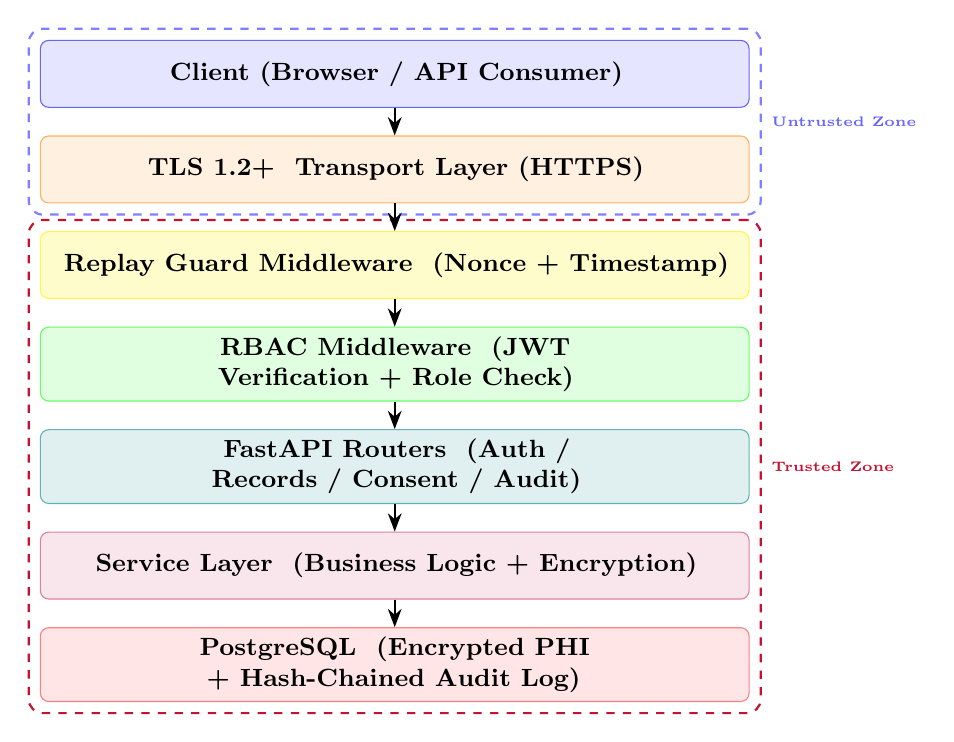
\begin{tikzpicture}[node distance=0.35cm]
  %% ── Nodes (stacked top-to-bottom) ──────────────────────────────────────
  \node[layer,fill=blue!10,draw=blue!60]   (client) {Client (Browser / API Consumer)};
  \node[layer,fill=orange!12,draw=orange!60,below=of client]  (tls)    {TLS 1.2+\ \ Transport Layer (HTTPS)};
  \node[layer,fill=yellow!20,draw=yellow!70,below=of tls]     (replay) {Replay Guard Middleware\ \ (Nonce + Timestamp)};
  \node[layer,fill=green!12,draw=green!60,below=of replay]    (rbac)   {RBAC Middleware\ \ (JWT Verification + Role Check)};
  \node[layer,fill=teal!12,draw=teal!60,below=of rbac]        (api)    {FastAPI Routers\ \ (Auth / Records / Consent / Audit)};
  \node[layer,fill=purple!10,draw=purple!50,below=of api]     (svc)    {Service Layer\ \ (Business Logic + Encryption)};
  \node[layer,fill=red!10,draw=red!50,below=of svc]           (db)     {PostgreSQL\ \ (Encrypted PHI + Hash-Chained Audit Log)};

  %% ── Arrows ──────────────────────────────────────────────────────────────
  \foreach \a/\b in {client/tls,tls/replay,replay/rbac,rbac/api,api/svc,svc/db}{
    \draw[arr] (\a.south)--(\b.north);
  }

  %% ── Trust boundary boxes ────────────────────────────────────────────────
  \begin{scope}[on background layer]
    \node[draw=blue!50,dashed,thick,rounded corners=5pt,
          fit=(client)(tls),inner sep=4pt,
          label={[font=\tiny\bfseries,text=blue!60]right:Untrusted Zone}] {};
    \node[draw=cmuRed,dashed,thick,rounded corners=5pt,
          fit=(replay)(rbac)(api)(svc)(db),inner sep=4pt,
          label={[font=\tiny\bfseries,text=cmuRed]right:Trusted Zone}] {};
  \end{scope}
\end{tikzpicture}
\caption{MedVault layered architecture with trust boundaries.}
\label{fig:layers}
\end{figure}

\subsection{Trust Boundaries}
\begin{description}[leftmargin=1.5em]
  \item[Untrusted Zone] Browsers, mobile clients, third-party integrations.
    All traffic is treated as hostile. TLS encrypts the channel; Replay Guard
    and RBAC validate every request before business logic runs.
  \item[Trusted Zone] The FastAPI process, service layer, and PostgreSQL on the
    same private network. Communication uses the asyncpg pool over a Unix socket
    or private LAN.
  \item[DB Privilege Boundary] The application DB role has \texttt{INSERT +
    SELECT} only on \texttt{audit\_log}, enforcing append-only semantics even
    if the application process is compromised.
\end{description}

\subsection{Module Interaction Diagram}

\begin{figure}[H]
\centering
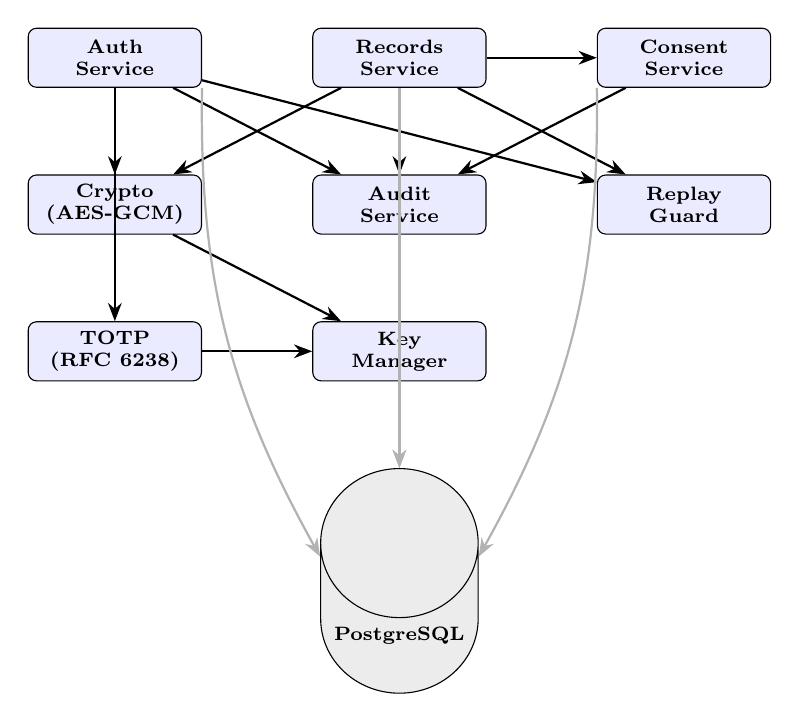
\begin{tikzpicture}[node distance=1.1cm and 1.4cm]
  %% Row 1
  \node[mod]                        (auth)    {Auth\\Service};
  \node[mod,right=of auth]          (records) {Records\\Service};
  \node[mod,right=of records]       (consent) {Consent\\Service};
  %% Row 2
  \node[mod,below=of auth]          (crypto)  {Crypto\\(AES-GCM)};
  \node[mod,below=of records]       (audit)   {Audit\\Service};
  \node[mod,below=of consent]       (replay)  {Replay\\Guard};
  %% Row 3
  \node[mod,below=of crypto]        (totp)    {TOTP\\(RFC 6238)};
  \node[mod,below=of audit]         (keymgr)  {Key\\Manager};
  %% DB
  \node[draw,cylinder,shape border rotate=90,
        minimum width=2cm,minimum height=0.9cm,
        font=\scriptsize\bfseries,fill=gray!15,
        below=of keymgr]            (pg)      {PostgreSQL};

  %% Edges
  \draw[arr](auth)--(crypto);
  \draw[arr](auth)--(totp);
  \draw[arr](auth)--(audit);
  \draw[arr](auth)--(replay);
  \draw[arr](records)--(crypto);
  \draw[arr](records)--(audit);
  \draw[arr](records)--(consent);
  \draw[arr](records)--(replay);
  \draw[arr](consent)--(audit);
  \draw[arr](crypto)--(keymgr);
  \draw[arr](totp)--(keymgr);
  \draw[darr](auth.south east) to[bend right=15] (pg.north west);
  \draw[darr](records.south) -- (pg.north);
  \draw[darr](consent.south west) to[bend left=15] (pg.north east);
  \draw[darr](audit.south) -- (pg.north);
\end{tikzpicture}
\caption{Module interaction. All services write to Audit; all crypto goes through Key Manager.}
\label{fig:modules}
\end{figure}

\subsection{Database Schema (Key Tables)}
\begin{center}
\begin{tabular}{lll}
  \toprule
  \textbf{Table} & \textbf{Key Columns} & \textbf{Security Note} \\
  \midrule
  \texttt{users}            & id, email, password\_hash, role        & bcrypt hash, no plaintext \\
  \texttt{mfa\_secrets}     & user\_id, encrypted\_secret, iv, tag   & AES-256-GCM \\
  \texttt{refresh\_tokens}  & token\_hash, user\_id, expires\_at     & SHA-256 hash only \\
  \texttt{medical\_records} & encrypted\_data, iv, tag, patient\_id  & AES-256-GCM per record \\
  \texttt{consent\_grants}  & doctor\_id, patient\_id, expires\_at   & time-limited \\
  \texttt{audit\_log}       & event\_type, actor\_id, chain\_hash    & append-only, hash-chained \\
  \texttt{nonce\_store}     & nonce, expires\_at                     & 5-min TTL \\
  \bottomrule
\end{tabular}
\end{center}

%% =============================================================================
\section{Threat Model}
%% =============================================================================

\subsection{Assets}
\begin{enumerate}[leftmargin=1.5em]
  \item \textbf{Protected Health Information (PHI)} -- diagnoses, lab results,
    treatment plans stored in \texttt{medical\_records}.
  \item \textbf{Authentication Credentials} -- passwords, TOTP secrets, JWT signing key.
  \item \textbf{Audit Trail} -- hash-chained log providing non-repudiation and tamper evidence.
  \item \textbf{Consent Grants} -- time-limited authorisations controlling doctor access.
  \item \textbf{Encryption Keys} -- \texttt{RECORD\_ENCRYPTION\_KEY} and
    \texttt{TOTP\_ENCRYPTION\_KEY} stored in environment variables.
\end{enumerate}

\subsection{Adversary Profiles}
\begin{center}
\begin{tabular}{p{3cm}p{4cm}p{5.5cm}}
  \toprule
  \textbf{Adversary} & \textbf{Capabilities} & \textbf{Goals} \\
  \midrule
  External attacker       & Network access, captured HTTP traffic & Steal PHI, forge tokens, replay requests \\
  Malicious insider       & Valid credentials, DB read access     & Escalate privileges, access unauthorised records \\
  Compromised DB admin    & Direct PostgreSQL access              & Modify audit log, read encrypted data \\
  Rogue doctor            & Valid JWT, no consent grant           & Access patient records without consent \\
  \bottomrule
\end{tabular}
\end{center}

\subsection{STRIDE Threat Analysis}

\begin{figure}[H]
\centering
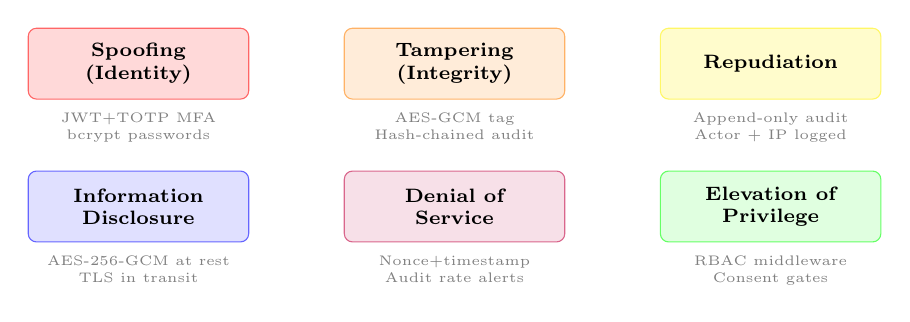
\begin{tikzpicture}[node distance=0.9cm and 1.2cm]
  %% Top row
  \node[threat,fill=red!15,draw=red!60]      (S) {Spoofing\\(Identity)};
  \node[threat,fill=orange!15,draw=orange!60,right=of S] (T) {Tampering\\(Integrity)};
  \node[threat,fill=yellow!20,draw=yellow!60,right=of T] (R) {Repudiation};
  %% Bottom row
  \node[threat,fill=blue!12,draw=blue!60,below=of S]     (I) {Information\\Disclosure};
  \node[threat,fill=purple!12,draw=purple!60,below=of T] (D) {Denial of\\Service};
  \node[threat,fill=green!12,draw=green!60,below=of R]   (E) {Elevation of\\Privilege};

  %% Mitigation labels
  \node[font=\tiny,text=gray,align=center,below=0.05cm of S]
    {JWT+TOTP MFA\\bcrypt passwords};
  \node[font=\tiny,text=gray,align=center,below=0.05cm of T]
    {AES-GCM tag\\Hash-chained audit};
  \node[font=\tiny,text=gray,align=center,below=0.05cm of R]
    {Append-only audit\\Actor + IP logged};
  \node[font=\tiny,text=gray,align=center,below=0.05cm of I]
    {AES-256-GCM at rest\\TLS in transit};
  \node[font=\tiny,text=gray,align=center,below=0.05cm of D]
    {Nonce+timestamp\\Audit rate alerts};
  \node[font=\tiny,text=gray,align=center,below=0.05cm of E]
    {RBAC middleware\\Consent gates};
\end{tikzpicture}
\caption{STRIDE threat categories and mitigations in MedVault.}
\label{fig:stride}
\end{figure}

\subsection{Risk Register}
\begin{longtable}{p{3.8cm}p{1.6cm}p{1.4cm}p{1.4cm}p{3.8cm}}
  \toprule
  \textbf{Threat} & \textbf{Likelihood} & \textbf{Impact} & \textbf{Risk} & \textbf{Mitigation} \\
  \midrule\endhead
  Credential theft / phishing  & High   & Critical & \textcolor{red}{\textbf{Critical}} & TOTP MFA; 15-min token expiry \\
  DB breach (PHI exposure)     & Medium & Critical & \textcolor{red}{\textbf{High}}     & AES-256-GCM field encryption \\
  Replay attack                & Medium & High     & \textcolor{orange}{\textbf{High}}  & Nonce + 5-min timestamp window \\
  Privilege escalation         & Low    & High     & \textcolor{orange}{\textbf{Medium}}& RBAC on every endpoint \\
  Audit log tampering          & Low    & Critical & \textcolor{orange}{\textbf{Medium}}& SHA-256 hash chain; DB INSERT-only \\
  Unauthorised record access   & Medium & High     & \textcolor{orange}{\textbf{High}}  & Consent grant check \\
  JWT forgery                  & Low    & Critical & \textcolor{orange}{\textbf{Medium}}& HMAC-SHA256 sig; short expiry \\
  Timing attack on TOTP        & Low    & Medium   & \textcolor{defenseGreen}{\textbf{Low}} & \texttt{hmac.compare\_digest()} \\
  \bottomrule
\end{longtable}

%% =============================================================================
\section{Secure Protocol Design}
%% =============================================================================

\subsection{Authentication Protocol}

The authentication flow combines password-based login with TOTP MFA and
short-lived JWT tokens. The full implementation is in
\srcref{app/services/auth\_service.py}{app/services/auth\_service.py}.

\begin{figure}[H]
\centering
%% Sequence diagram drawn as a simple message-passing table in TikZ
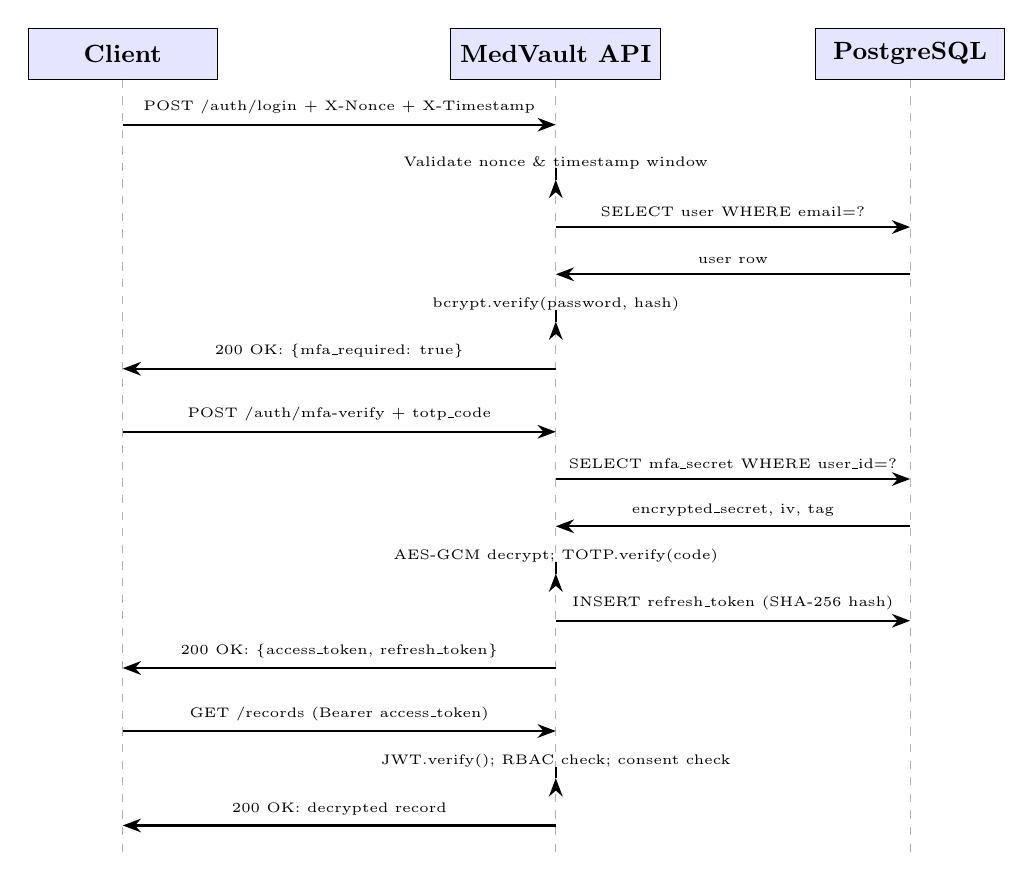
\begin{tikzpicture}[
  actor/.style={draw,fill=blue!10,minimum width=2.4cm,minimum height=0.65cm,
                font=\small\bfseries,align=center},
  lbl/.style={font=\tiny,align=center},
  every node/.style={font=\small},
]
  %% ── Actor headers ────────────────────────────────────────────────────────
  \node[actor] (C) at (0,0)   {Client};
  \node[actor] (S) at (5.5,0) {MedVault API};
  \node[actor] (D) at (10,0)  {PostgreSQL};

  %% ── Lifelines ────────────────────────────────────────────────────────────
  \draw[dashed,gray!60] (0,-0.33)   -- (0,-10.2);
  \draw[dashed,gray!60] (5.5,-0.33) -- (5.5,-10.2);
  \draw[dashed,gray!60] (10,-0.33)  -- (10,-10.2);

  %% ── Messages ─────────────────────────────────────────────────────────────
  \draw[arr](0,-0.9)  -- node[above,lbl]{POST /auth/login + X-Nonce + X-Timestamp}(5.5,-0.9);
  \draw[arr](5.5,-1.6)-- node[above,lbl]{Validate nonce \& timestamp window}(5.5,-1.6);
  \draw[arr](5.5,-2.2)-- node[above,lbl]{SELECT user WHERE email=?}(10,-2.2);
  \draw[arr](10,-2.8) -- node[above,lbl]{user row}(5.5,-2.8);
  \draw[arr](5.5,-3.4)-- node[above,lbl]{bcrypt.verify(password, hash)}(5.5,-3.4);
  \draw[arr](5.5,-4.0)-- node[above,lbl]{200 OK: \{mfa\_required: true\}}(0,-4.0);

  \draw[arr](0,-4.8)  -- node[above,lbl]{POST /auth/mfa-verify + totp\_code}(5.5,-4.8);
  \draw[arr](5.5,-5.4)-- node[above,lbl]{SELECT mfa\_secret WHERE user\_id=?}(10,-5.4);
  \draw[arr](10,-6.0) -- node[above,lbl]{encrypted\_secret, iv, tag}(5.5,-6.0);
  \draw[arr](5.5,-6.6)-- node[above,lbl]{AES-GCM decrypt; TOTP.verify(code)}(5.5,-6.6);
  \draw[arr](5.5,-7.2)-- node[above,lbl]{INSERT refresh\_token (SHA-256 hash)}(10,-7.2);
  \draw[arr](5.5,-7.8)-- node[above,lbl]{200 OK: \{access\_token, refresh\_token\}}(0,-7.8);

  \draw[arr](0,-8.6)  -- node[above,lbl]{GET /records (Bearer access\_token)}(5.5,-8.6);
  \draw[arr](5.5,-9.2)-- node[above,lbl]{JWT.verify(); RBAC check; consent check}(5.5,-9.2);
  \draw[arr](5.5,-9.8)-- node[above,lbl]{200 OK: decrypted record}(0,-9.8);
\end{tikzpicture}
\caption{Authentication sequence: login $\to$ TOTP MFA $\to$ JWT issuance $\to$ protected resource.}
\label{fig:authflow}
\end{figure}

\subsection{Key Exchange and Token Lifecycle}
\begin{itemize}[leftmargin=1.5em]
  \item \textbf{Access tokens} -- HS256 JWTs signed with \texttt{JWT\_SECRET\_KEY},
    valid for 15 minutes.
    See \srcref{app/middleware/rbac.py}{app/middleware/rbac.py}.
  \item \textbf{Refresh tokens} -- 32-byte random values; only their SHA-256 hash
    is stored. Rotated on every use; old token immediately invalidated.
  \item \textbf{TOTP secrets} -- generated with \texttt{os.urandom(20)}, stored
    encrypted with AES-256-GCM under a dedicated \texttt{TOTP\_ENCRYPTION\_KEY}.
    See \srcref{app/core/totp.py}{app/core/totp.py}.
\end{itemize}

\subsection{Replay Attack Prevention}

Every sensitive endpoint requires two headers validated by
\srcref{app/middleware/replay\_guard.py}{app/middleware/replay\_guard.py}:

\begin{center}
\begin{tabular}{lll}
  \toprule
  \textbf{Header} & \textbf{Format} & \textbf{Validation} \\
  \midrule
  \texttt{X-Nonce}     & UUID v4 string & Must not appear in \texttt{nonce\_store} (5-min TTL) \\
  \texttt{X-Timestamp} & ISO-8601 UTC   & Must be within $\pm$5 min of server time \\
  \bottomrule
\end{tabular}
\end{center}

\begin{figure}[H]
\centering
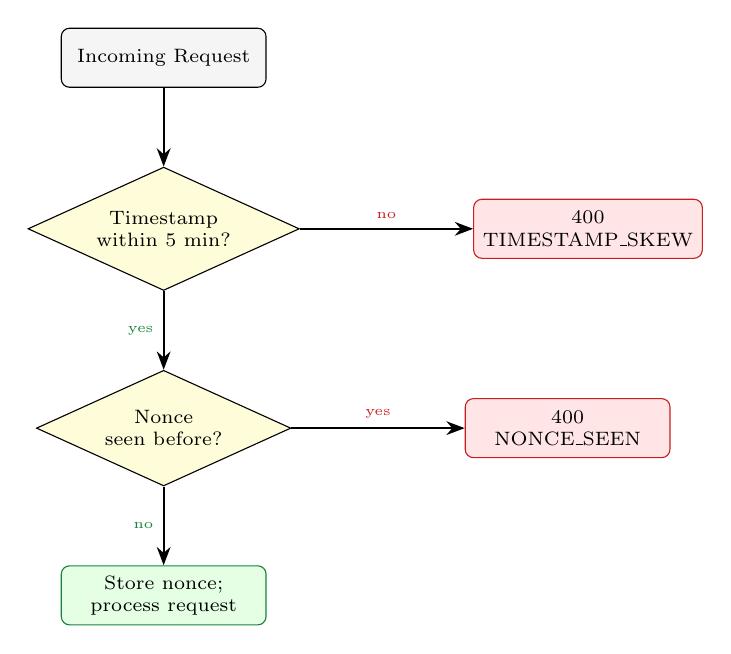
\begin{tikzpicture}[node distance=1.0cm and 2.2cm]
  \node[sbox]                              (req)   {Incoming Request};
  \node[diam,below=of req]                 (ts)    {Timestamp\\within 5 min?};
  \node[diam,below=of ts]                  (nonce) {Nonce\\seen before?};
  \node[sbox,fill=green!10,draw=defenseGreen,below=of nonce] (ok) {Store nonce;\\ process request};
  \node[sbox,fill=red!10,draw=attackRed,right=of ts]         (r1) {400\\TIMESTAMP\_SKEW};
  \node[sbox,fill=red!10,draw=attackRed,right=of nonce]      (r2) {400\\NONCE\_SEEN};

  \draw[arr](req)--(ts);
  \draw[arr](ts)    -- node[left,font=\tiny,text=defenseGreen]{yes}(nonce);
  \draw[arr](ts)    -- node[above,font=\tiny,text=attackRed]{no} (r1);
  \draw[arr](nonce) -- node[left,font=\tiny,text=defenseGreen]{no} (ok);
  \draw[arr](nonce) -- node[above,font=\tiny,text=attackRed]{yes}(r2);
\end{tikzpicture}
\caption{Replay Guard middleware decision flow.}
\label{fig:replayguard}
\end{figure}

\subsection{Encryption Design}

\subsubsection{AES-256-GCM Field-Level Encryption}

Every medical record is encrypted individually before storage. The full
implementation is in \srcref{app/core/crypto.py}{app/core/crypto.py}.

Key design decisions:
\begin{itemize}[leftmargin=1.5em]
  \item \textbf{Random 12-byte IV per operation} -- prevents IV reuse, which
    would catastrophically break GCM confidentiality.
  \item \textbf{Authenticated encryption} -- the 128-bit GCM tag covers the
    entire ciphertext, detecting any modification.
  \item \textbf{Separate keys} -- \texttt{RECORD\_ENCRYPTION\_KEY} $\neq$
    \texttt{TOTP\_ENCRYPTION\_KEY}; a compromised record key does not expose
    TOTP secrets. See \srcref{app/core/key\_manager.py}{app/core/key\_manager.py}.
\end{itemize}

\subsubsection{Custom TOTP (RFC 6238)}

The TOTP module uses only Python stdlib (\texttt{hmac}, \texttt{hashlib},
\texttt{struct}, \texttt{time}, \texttt{os}, \texttt{base64}) -- no
third-party dependency. Full source:
\srcref{app/core/totp.py}{app/core/totp.py}.

\subsection{Audit Chain Algorithm}

The audit log uses a SHA-256 linked list for tamper evidence. Full source:
\srcref{app/services/audit\_service.py}{app/services/audit\_service.py}.

\begin{figure}[H]
\centering
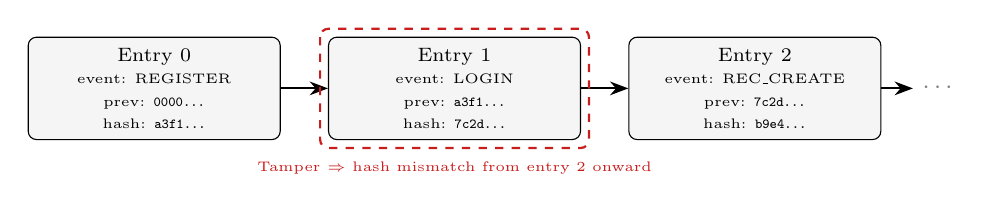
\begin{tikzpicture}[node distance=0.6cm and 0.5cm]
  \node[sbox,minimum width=3.2cm,minimum height=1.3cm,align=center] (e0)
    {Entry 0\\{\tiny event: REGISTER}\\{\tiny prev: \texttt{0000\ldots}}\\{\tiny hash: \texttt{a3f1\ldots}}};
  \node[sbox,minimum width=3.2cm,minimum height=1.3cm,align=center,right=0.6cm of e0] (e1)
    {Entry 1\\{\tiny event: LOGIN}\\{\tiny prev: \texttt{a3f1\ldots}}\\{\tiny hash: \texttt{7c2d\ldots}}};
  \node[sbox,minimum width=3.2cm,minimum height=1.3cm,align=center,right=0.6cm of e1] (e2)
    {Entry 2\\{\tiny event: REC\_CREATE}\\{\tiny prev: \texttt{7c2d\ldots}}\\{\tiny hash: \texttt{b9e4\ldots}}};
  \node[font=\small,text=gray,right=0.4cm of e2] (dots) {$\cdots$};

  \draw[arr](e0.east)--(e1.west);
  \draw[arr](e1.east)--(e2.west);
  \draw[arr](e2.east)--(dots.west);

  \draw[attackRed,dashed,thick,rounded corners=3pt]
    ($(e1.north west)+(-0.1,0.1)$) rectangle ($(e1.south east)+(0.1,-0.1)$);
  \node[text=attackRed,font=\tiny,below=0.15cm of e1]
    {Tamper $\Rightarrow$ hash mismatch from entry~2 onward};
\end{tikzpicture}
\caption{SHA-256 hash-chained audit log. Any modification breaks all subsequent hashes.}
\label{fig:auditchain}
\end{figure}

\subsection{Consent Protocol}

Full implementation: \srcref{app/services/consent\_service.py}{app/services/consent\_service.py}.

\begin{figure}[H]
\centering
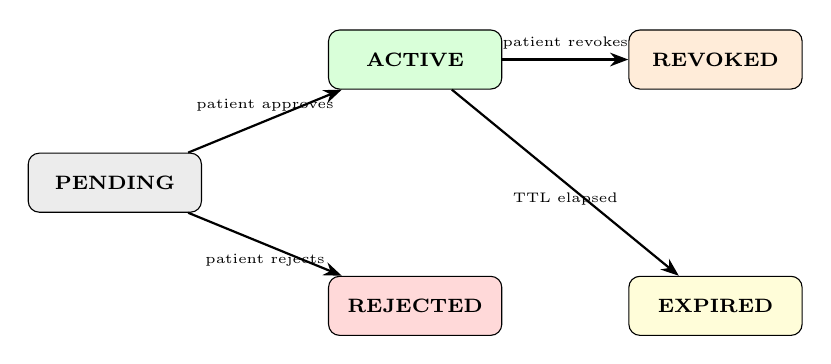
\begin{tikzpicture}[node distance=0.8cm and 1.6cm]
  \node[state,fill=gray!15]   (pending)  {PENDING};
  \node[state,fill=green!15,  above right=of pending] (active)   {ACTIVE};
  \node[state,fill=red!15,    below right=of pending] (rejected) {REJECTED};
  \node[state,fill=orange!15, right=of active]        (revoked)  {REVOKED};
  \node[state,fill=yellow!15, right=of rejected]      (expired)  {EXPIRED};

  \draw[arr](pending) -- node[above,font=\tiny]{patient approves}(active);
  \draw[arr](pending) -- node[below,font=\tiny]{patient rejects} (rejected);
  \draw[arr](active)  -- node[above,font=\tiny]{patient revokes} (revoked);
  \draw[arr](active)  -- node[below,font=\tiny]{TTL elapsed}     (expired);
\end{tikzpicture}
\caption{Consent grant state machine. Doctors may only access records while a grant is ACTIVE.}
\label{fig:consent}
\end{figure}

%% =============================================================================
\section{Working Prototype}
%% =============================================================================

\subsection{Implementation Overview}

The MedVault backend is a fully functional FastAPI application with 8 routers,
12 database tables, and 20+ API endpoints. All 13 formal requirements from the
design specification have been implemented and tested.

%% INSERT PHOTO HERE
%% Type: screenshot of FastAPI Swagger UI (/docs)
%% Caption suggestion: "Auto-generated OpenAPI documentation showing all endpoints"

\subsection{Project Structure}

The repository layout is shown below. Each path is a direct link to the source:

\begin{center}
\begin{tabular}{ll}
  \toprule
  \textbf{Path} & \textbf{Purpose} \\
  \midrule
  \srcref{app/main.py}{app/main.py}                           & FastAPI app setup, router registration \\
  \srcref{app/core/crypto.py}{app/core/crypto.py}             & AES-256-GCM encrypt / decrypt \\
  \srcref{app/core/totp.py}{app/core/totp.py}                 & RFC 6238 TOTP (stdlib only) \\
  \srcref{app/core/key\_manager.py}{app/core/key\_manager.py} & Key loading and startup validation \\
  \srcref{app/middleware/rbac.py}{app/middleware/rbac.py}      & JWT verification + role enforcement \\
  \srcref{app/middleware/replay\_guard.py}{app/middleware/replay\_guard.py} & Nonce + timestamp validation \\
  \srcref{app/services/auth\_service.py}{app/services/auth\_service.py}     & Registration, login, MFA, token refresh \\
  \srcref{app/services/records\_service.py}{app/services/records\_service.py} & CRUD with encryption and access control \\
  \srcref{app/services/consent\_service.py}{app/services/consent\_service.py} & Consent request / approval / revocation \\
  \srcref{app/services/audit\_service.py}{app/services/audit\_service.py}   & Append, verify chain, list entries \\
  \srcref{attacks/}{attacks/}                                 & 11 attack demonstration scripts \\
  \srcref{tests/}{tests/}                                     & pytest + Hypothesis test suites \\
  \srcref{alembic/versions/}{alembic/versions/}               & 9 database migration scripts \\
  \bottomrule
\end{tabular}
\end{center}

\subsection{API Endpoints}

\begin{center}
\begin{longtable}{p{1.6cm}p{5.2cm}p{2.4cm}p{3cm}}
  \toprule
  \textbf{Method} & \textbf{Endpoint} & \textbf{Auth} & \textbf{Role} \\
  \midrule\endhead
  POST   & /auth/register               & None         & Public \\
  POST   & /auth/login                  & Nonce+TS     & Public \\
  POST   & /auth/mfa-verify             & None         & Public \\
  POST   & /auth/refresh                & Refresh token& Any \\
  POST   & /auth/logout                 & JWT          & Any \\
  POST   & /auth/password-reset-request & Nonce+TS     & Public \\
  POST   & /auth/password-reset-confirm & Nonce+TS     & Public \\
  GET    & /users/me                    & JWT          & Any \\
  \midrule
  POST   & /records                     & JWT+Nonce+TS & Doctor/Nurse/Lab \\
  GET    & /records                     & JWT          & Any (filtered) \\
  GET    & /records/\{id\}              & JWT          & Any (consent check) \\
  PUT    & /records/\{id\}              & JWT+Nonce+TS & Doctor/Nurse/Lab \\
  DELETE & /records/\{id\}              & JWT+Nonce+TS & Doctor/Admin \\
  \midrule
  POST   & /consent                     & JWT+Nonce+TS & Doctor \\
  POST   & /consent/\{id\}/approve      & JWT          & Patient \\
  POST   & /consent/\{id\}/reject       & JWT          & Patient \\
  POST   & /consent/\{id\}/revoke       & JWT          & Patient \\
  GET    & /consent                     & JWT          & Any (filtered) \\
  \midrule
  GET    & /audit                       & JWT          & Admin / Patient (scoped) \\
  GET    & /audit/verify                & JWT          & Admin / Patient (scoped) \\
  \bottomrule
\end{longtable}
\end{center}

\subsection{Key Implementation Highlights}

\begin{description}[leftmargin=1.5em]
  \item[RBAC Middleware]
    Every protected endpoint is decorated with \texttt{require\_roles()}.
    The decorator decodes the JWT, extracts the role claim, and returns
    \texttt{403 Forbidden} if the role is not in the allowed set.
    Source: \srcref{app/middleware/rbac.py}{app/middleware/rbac.py}.

  \item[Consent Gate]
    \texttt{\_can\_read()} in the records service queries \texttt{consent\_grants}
    for an active, non-expired grant before allowing a Doctor to read a record.
    Source: \srcref{app/services/records\_service.py}{app/services/records\_service.py}.

  \item[Audit Append]
    Every sensitive action calls \texttt{audit\_service.append()}, which
    computes the SHA-256 hash over the new entry concatenated with the previous
    entry's hash, forming the chain.
    Source: \srcref{app/services/audit\_service.py}{app/services/audit\_service.py}.
\end{description}

\subsection{Testing}
\begin{center}
\begin{tabular}{lll}
  \toprule
  \textbf{Suite} & \textbf{Coverage} & \textbf{Source} \\
  \midrule
  TOTP unit tests      & RFC 6238 compliance, timing resistance & \srcref{tests/unit/test\_totp.py}{tests/unit/test\_totp.py} \\
  Crypto unit tests    & AES-GCM round-trip, IV uniqueness      & \srcref{tests/unit/test\_crypto.py}{tests/unit/test\_crypto.py} \\
  Audit chain tests    & Hash integrity, tamper detection       & \srcref{tests/unit/test\_audit\_chain.py}{tests/unit/test\_audit\_chain.py} \\
  RBAC tests           & Role enforcement, JWT validation       & \srcref{tests/unit/test\_rbac.py}{tests/unit/test\_rbac.py} \\
  Attack scenario tests& All 11 attack/defence pairs            & \srcref{tests/unit/test\_attack\_scenarios.py}{tests/unit/test\_attack\_scenarios.py} \\
  Property-based tests & TOTP window, audit chain properties    & Hypothesis (all suites) \\
  \bottomrule
\end{tabular}
\end{center}

%% =============================================================================
\section{Attack \& Defence Demonstrations}
%% =============================================================================

All attack scripts live in \srcref{attacks/}{attacks/} and share utilities
from \srcref{attacks/shared.py}{attacks/shared.py}. The full manual demo guide
is in \srcref{ATTACKS.md}{ATTACKS.md}.

%% INSERT PHOTO HERE
%% Type: terminal screenshot of any attack script running
%% Caption suggestion: "Terminal output of the replay attack demo showing BLOCKED response"

\subsection{Attack 1 -- Replay Attack}
\begin{attackbox}
Attacker captures a valid login request (headers + body + nonce) and re-sends
it to obtain a second authentication token.
Source: \srcref{attacks/01\_replay\_attack.py}{attacks/01\_replay\_attack.py}.
\end{attackbox}
\begin{defensebox}
\texttt{replay\_guard} stores every nonce in \texttt{nonce\_store} (5-min TTL).
A duplicate nonce is rejected with \texttt{400 REPLAY\_NONCE\_SEEN} before any
authentication logic runs.
Source: \srcref{app/middleware/replay\_guard.py}{app/middleware/replay\_guard.py}.
\end{defensebox}

\subsection{Attack 2 -- Stale Timestamp Rejection}
\begin{attackbox}
Attacker replays a request with a timestamp from the distant past
(e.g.\ \texttt{2020-01-01T00:00:00Z}).
Source: \srcref{attacks/02\_stale\_timestamp.py}{attacks/02\_stale\_timestamp.py}.
\end{attackbox}
\begin{defensebox}
Timestamp must be within $\pm$5 minutes of server time.
Returns \texttt{400 REPLAY\_TIMESTAMP\_SKEW}.
\end{defensebox}

\subsection{Attack 3 -- Privilege Escalation (Patient $\to$ Doctor)}
\begin{attackbox}
A Patient-role user sends \texttt{POST /records} (a Doctor-only action) using
their own valid JWT.
Source: \srcref{attacks/03\_privilege\_escalation.py}{attacks/03\_privilege\_escalation.py}.
\end{attackbox}
\begin{defensebox}
\texttt{require\_roles("Doctor","Nurse","Lab\_Technician")} on the endpoint
returns \texttt{403 Forbidden} before the handler executes.
Source: \srcref{app/middleware/rbac.py}{app/middleware/rbac.py}.
\end{defensebox}

\subsection{Attack 4 -- User Enumeration}
\begin{attackbox}
Attacker probes the login endpoint with different email addresses, hoping to
distinguish ``email not found'' from ``wrong password'' responses.
Source: \srcref{attacks/04\_jwt\_forgery.py}{attacks/04\_jwt\_forgery.py}.
\end{attackbox}
\begin{defensebox}
Both cases return the identical body:
\texttt{\{"detail":"Invalid credentials","error\_code":"INVALID\_CREDENTIALS"\}}.
Source: \srcref{app/services/auth\_service.py}{app/services/auth\_service.py}.
\end{defensebox}

\subsection{Attack 5 -- Brute Force Detection}
\begin{attackbox}
Attacker tries multiple passwords against a known account in rapid succession.
Source: \srcref{attacks/05\_user\_enumeration.py}{attacks/05\_user\_enumeration.py}.
\end{attackbox}
\begin{defensebox}
Every failed login is logged as \texttt{LOGIN\_FAILED} in the audit trail with
the actor's IP. Administrators query the audit log to detect and respond to
brute-force patterns.
Source: \srcref{app/services/auth\_service.py}{app/services/auth\_service.py}.
\end{defensebox}

\subsection{Attack 6 -- Audit Log Tampering}
\begin{attackbox}
Attacker with direct PostgreSQL access modifies an audit entry to hide their
actions (e.g.\ \texttt{UPDATE audit\_log SET event\_type = 'TAMPERED' WHERE id = 1}).
Source: \srcref{attacks/07\_audit\_tampering.py}{attacks/07\_audit\_tampering.py}.
\end{attackbox}
\begin{defensebox}
The SHA-256 hash chain detects the modification. \texttt{GET /audit/verify}
recomputes every hash and reports the first broken link.
Source: \srcref{app/services/audit\_service.py}{app/services/audit\_service.py}.
\end{defensebox}

\begin{figure}[H]
\centering
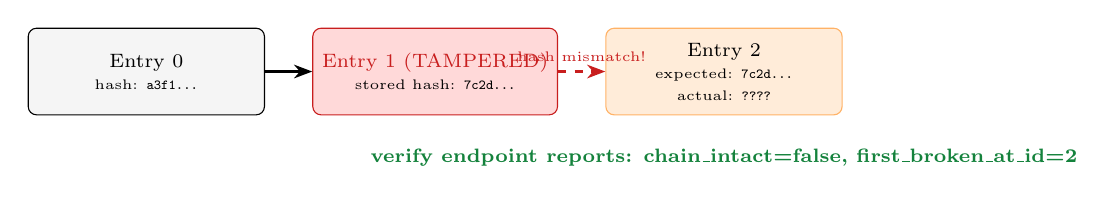
\begin{tikzpicture}[node distance=0.5cm and 0.6cm]
  \node[sbox,minimum width=3cm,minimum height=1.1cm,align=center] (e0)
    {Entry 0\\{\tiny hash: \texttt{a3f1\ldots}}};
  \node[sbox,minimum width=3cm,minimum height=1.1cm,align=center,
        fill=red!15,draw=attackRed,right=0.6cm of e0] (e1)
    {\textcolor{attackRed}{Entry 1 (TAMPERED)}\\{\tiny stored hash: \texttt{7c2d\ldots}}};
  \node[sbox,minimum width=3cm,minimum height=1.1cm,align=center,
        fill=orange!15,draw=orange!60,right=0.6cm of e1] (e2)
    {Entry 2\\{\tiny expected: \texttt{7c2d\ldots}}\\{\tiny actual: \texttt{????}}};

  \draw[arr](e0.east)--(e1.west);
  \draw[-Stealth,thick,attackRed,dashed](e1.east)
    -- node[above,font=\tiny,text=attackRed]{hash mismatch!}(e2.west);

  \node[text=defenseGreen,font=\scriptsize\bfseries,below=0.3cm of e2]
    {verify endpoint reports: chain\_intact=false, first\_broken\_at\_id=2};
\end{tikzpicture}
\caption{Audit chain tamper detection: modifying entry 1 breaks the hash at entry 2.}
\label{fig:tamper}
\end{figure}

\subsection{Attack 7 -- Unauthorised Record Access (No Consent)}
\begin{attackbox}
A Doctor with a valid JWT but no active consent grant attempts to read a
patient's records.
Source: \srcref{attacks/08\_unauthorized\_record\_access.py}{attacks/08\_unauthorized\_record\_access.py}.
\end{attackbox}
\begin{defensebox}
\texttt{\_can\_read()} queries \texttt{consent\_grants} for an active,
non-expired grant. Without one, returns \texttt{403 Forbidden} and logs
\texttt{ACCESS\_DENIED}.
Source: \srcref{app/services/records\_service.py}{app/services/records\_service.py}.
\end{defensebox}

\subsection{Attack 8 -- Cross-Patient Access}
\begin{attackbox}
A Patient-role user supplies a different \texttt{patient\_id} in the query to
read another patient's records.
Source: \srcref{attacks/09\_cross\_patient\_access.py}{attacks/09\_cross\_patient\_access.py}.
\end{attackbox}
\begin{defensebox}
\texttt{\_can\_read()} checks \texttt{record.patient\_id == user\_id} for
Patient-role requests. Mismatches return \texttt{403 Forbidden}.
\end{defensebox}

\subsection{Attack 9 -- Draft Record Leakage}
\begin{attackbox}
A patient attempts to read a record saved as a draft (not yet published).
Source: \srcref{attacks/10\_draft\_record\_leakage.py}{attacks/10\_draft\_record\_leakage.py}.
\end{attackbox}
\begin{defensebox}
The records service filters by \texttt{status == "published"} for Patient-role
requests. Draft records are invisible to patients until explicitly published.
\end{defensebox}

\subsection{Attack 10 -- AES-GCM Ciphertext Tampering}
\begin{attackbox}
Attacker with DB access flips a byte in the \texttt{encrypted\_data} column of
\texttt{medical\_records}, hoping to alter a diagnosis undetected (as would be
possible with AES-CBC).
Source: \srcref{attacks/11\_aes\_gcm\_tampering.py}{attacks/11\_aes\_gcm\_tampering.py}.
See also: \srcref{attacks/11\_aes\_gcm\_tampering.md}{attacks/11\_aes\_gcm\_tampering.md}.
\end{attackbox}
\begin{defensebox}
AES-256-GCM provides \emph{authenticated encryption}. The 128-bit GCM tag
covers the entire ciphertext. Any modification raises \texttt{InvalidTag}
during decryption, returning \texttt{500} (which in production triggers an alert).
Source: \srcref{app/core/crypto.py}{app/core/crypto.py}.
\end{defensebox}

%% INSERT PHOTO HERE
%% Type: psql terminal screenshot showing the byte-flip UPDATE and the resulting 500 error
%% Caption suggestion: "PostgreSQL session: byte-flip tampering causes AES-GCM tag failure"

\subsection{Attack 11 -- Token Theft / Expired Token}
\begin{attackbox}
Attacker steals a JWT access token (e.g.\ from browser storage) and uses it
after the legitimate session ends.
\end{attackbox}
\begin{defensebox}
Access tokens expire after 15 minutes. Refresh tokens are rotated on each use;
the old token is immediately invalidated in the database.
Source: \srcref{app/services/auth\_service.py}{app/services/auth\_service.py}.
\end{defensebox}

\subsection{Summary}
\begin{longtable}{p{4cm}p{4.5cm}p{4cm}}
  \toprule
  \textbf{Attack} & \textbf{Defence} & \textbf{Source File} \\
  \midrule\endhead
  Replay attack          & Nonce + timestamp validation      & \texttt{middleware/replay\_guard.py} \\
  Stale timestamp        & $\pm$5-min window check           & \texttt{middleware/replay\_guard.py} \\
  Privilege escalation   & \texttt{require\_roles()} decorator & \texttt{middleware/rbac.py} \\
  User enumeration       & Identical error responses         & \texttt{services/auth\_service.py} \\
  Brute force            & \texttt{LOGIN\_FAILED} audit events & \texttt{services/auth\_service.py} \\
  Audit tampering        & SHA-256 hash chain                & \texttt{services/audit\_service.py} \\
  Unauthorised access    & Consent grant check               & \texttt{services/records\_service.py} \\
  Cross-patient access   & \texttt{patient\_id} ownership check & \texttt{services/records\_service.py} \\
  Draft record leakage   & \texttt{status == "published"} filter & \texttt{services/records\_service.py} \\
  AES-GCM tampering      & GCM authentication tag            & \texttt{core/crypto.py} \\
  Token theft            & 15-min expiry + refresh rotation  & \texttt{services/auth\_service.py} \\
  Timing attack (TOTP)   & \texttt{hmac.compare\_digest()}   & \texttt{core/totp.py} \\
  \bottomrule
\end{longtable}

%% =============================================================================
\section{Security Design Decisions}
%% =============================================================================

\begin{longtable}{p{3.8cm}p{3.2cm}p{5.5cm}}
  \toprule
  \textbf{Decision} & \textbf{Alternative} & \textbf{Justification} \\
  \midrule\endhead
  AES-256-GCM for PHI
    & AES-256-CBC + HMAC
    & GCM provides authenticated encryption in one primitive; CBC is vulnerable
      to padding oracle attacks and requires a separate MAC. \\
  \addlinespace
  Random 12-byte IV per operation
    & Deterministic IV
    & IV reuse in GCM is catastrophic (reveals keystream); random IV eliminates
      this risk entirely. \\
  \addlinespace
  Custom TOTP (stdlib only)
    & \texttt{pyotp} library
    & Reduces supply-chain attack surface; demonstrates RFC~6238 compliance
      from first principles. \\
  \addlinespace
  \texttt{hmac.compare\_digest()} for TOTP
    & String equality \texttt{==}
    & Constant-time comparison prevents timing side-channel attacks. \\
  \addlinespace
  SHA-256 hash-chained audit
    & Append-only table only
    & Hash chain makes tampering detectable even by the patient; a plain
      append-only table can be silently truncated by a DB admin. \\
  \addlinespace
  DB-level INSERT+SELECT on audit\_log
    & Application-level enforcement
    & Prevents application-layer bypass; even a compromised app process cannot
      delete audit entries. \\
  \addlinespace
  Separate RECORD and TOTP keys
    & Single master key
    & Limits blast radius: a compromised record key does not expose TOTP secrets. \\
  \addlinespace
  15-min JWT access token expiry
    & Long-lived tokens
    & Limits the window of opportunity for a stolen token. \\
  \addlinespace
  Refresh token rotation
    & Static refresh tokens
    & A stolen refresh token can only be used once before it is invalidated. \\
  \addlinespace
  Identical error for wrong email/password
    & Distinct error messages
    & Prevents user enumeration by external attackers. \\
  \bottomrule
\end{longtable}

%% =============================================================================
\section{Conclusion}
%% =============================================================================

MedVault demonstrates a complete, production-grade implementation of a secure
medical records system. The project satisfies all five course requirements:

\begin{enumerate}[leftmargin=1.5em]
  \item \textbf{System Architecture} -- Layered design with explicit trust
    boundaries, documented with TikZ diagrams.
  \item \textbf{Threat Model} -- STRIDE analysis covering 12 threat categories
    with a risk register and mitigations.
  \item \textbf{Secure Protocol Design} -- JWT + TOTP MFA, AES-256-GCM
    field-level encryption, SHA-256 hash-chained audit, and nonce-based replay
    prevention.
  \item \textbf{Working Prototype} -- Fully functional FastAPI backend with 20+
    endpoints, 12 database tables, and comprehensive test coverage.
  \item \textbf{Attack \& Defence Demo} -- 11 automated attack scenarios with
    corresponding defences, each with a Python script and documentation.
\end{enumerate}

The system applies \emph{defence in depth}: no single control is relied upon
exclusively. Transport (TLS), authentication (JWT+TOTP), authorisation
(RBAC + consent), encryption (AES-256-GCM), and audit (hash chain) each
provide an independent layer of protection.

\begin{notebox}
To run the system locally: copy \texttt{.env.example} to \texttt{.env},
generate keys (\texttt{openssl rand -hex 32}), then start with:\\[4pt]
\texttt{uvicorn app.main:app --ssl-certfile cert.pem --ssl-keyfile key.pem
--host 0.0.0.0 --port 8000}\\[4pt]
Run all tests with: \texttt{pytest tests/unit/ -v --tb=short}
\end{notebox}

%% =============================================================================
\appendix
\section{Environment Variables Reference}
%% =============================================================================

\begin{center}
\begin{tabular}{p{5.5cm}p{7cm}}
  \toprule
  \textbf{Variable} & \textbf{Description} \\
  \midrule
  \texttt{DATABASE\_URL}                  & PostgreSQL connection string (asyncpg) \\
  \texttt{JWT\_SECRET\_KEY}               & HS256 signing key (32+ random bytes) \\
  \texttt{JWT\_ALGORITHM}                 & HS256 (default) \\
  \texttt{RECORD\_ENCRYPTION\_KEY}        & AES-256 key for PHI (64 hex chars) \\
  \texttt{TOTP\_ENCRYPTION\_KEY}          & AES-256 key for TOTP secrets (64 hex chars) \\
  \texttt{ACCESS\_TOKEN\_EXPIRE\_MINUTES} & JWT access token lifetime (default: 15) \\
  \texttt{REFRESH\_TOKEN\_EXPIRE\_DAYS}   & Refresh token lifetime (default: 7) \\
  \texttt{DEV\_MODE}                      & Expose reset tokens in responses (dev only) \\
  \texttt{TLS\_CERT\_FILE}                & Path to TLS certificate \\
  \texttt{TLS\_KEY\_FILE}                 & Path to TLS private key \\
  \bottomrule
\end{tabular}
\end{center}
See \srcref{.env.example}{.env.example} for the full annotated template.

\end{document}
